%% Standalone lecture -- build with:  pdflatex -shell-escape entropy
%% Shared preamble for standalone lecture files.
%%
%% Every lecture begins with %% Shared preamble for standalone lecture files.
%%
%% Every lecture begins with %% Shared preamble for standalone lecture files.
%%
%% Every lecture begins with \input{preamble} and is compiled on its own:
%%     pdflatex -shell-escape <lecture>
%% There is no master lectures.tex any more -- the list of lectures lives in
%% lectures.yaml and is read by the build scripts.

\documentclass[25pt,landscape,footrule]{foils}
\input{macros_gen}
\backgroundsetup{contents={}}

\usepackage{stmaryrd}
\usepackage{ifthen}
\usepackage{pdf14}

% Every figure lives in this course's lectures/figures (consolidated
% 2026-10-08).  Do not add other courses' folders back: when a name exists in
% several folders LaTeX silently takes the first, which mixed old and new
% frames of the same animation.  A missing figure should be a build error.
\graphicspath{{figures/}{../lectures/figures/}}

\date{}

\newcounter{lessoncnt}
\newcommand{\lesson}[1]{\setcounter{page}{1}%
\section{Mathematics of Machine Learning\\%
\vfill
\textcolor{red}{\textit{#1}}
\vfill}}
 and is compiled on its own:
%%     pdflatex -shell-escape <lecture>
%% There is no master lectures.tex any more -- the list of lectures lives in
%% lectures.yaml and is read by the build scripts.

\documentclass[25pt,landscape,footrule]{foils}
%\usepackage[compat2,pdftex]{geometry}
\usepackage[pdftex]{geometry}
\geometry{headsep=-2.5ex,hscale=0.9,bmargin=2.5cm,tmargin=1cm,textwidth=25cm}
\usepackage[pdftex]{xcolor}
\usepackage{pause}
\usepackage{background}
%\usepackage[color=white]{background}
\usepackage{listings}
\usepackage{graphicx}
\usepackage{epsfig}
\usepackage{epstopdf}
\usepackage{bm}
\usepackage{amssymb}
\usepackage{amsfonts}
\usepackage{marvosym}
\usepackage{cite}
\usepackage{pifont}
\usepackage[english]{babel}
\usepackage{amsmath}
\usepackage{amsfonts}
\usepackage{rotating}
\usepackage{listings}
\usepackage{pp4slide}
%\usepackage{hyperref}
\usepackage{pp4link}
\usepackage{fancyvrb}
\usepackage{multido}
\usepackage{calc}
\usepackage{mleftright}
\mleftright % Redefines \left to \mleft and \right to \mright



\thinmuskip=1mu

\newcommand{\bigstrut}{\rule[-0.5\baselineskip]{0pt}{1.2\baselineskip}}
\renewcommand{\ttdefault}{pcr}

\newcommand{\squeeze}{\setlength{\itemsep}{-2pt}}
%\renewcommand{\familydefault}{cmr}
%\renewcommand{\labelitemii}{\textcolor{green}{$\star$}}
\newcommand{\tick}{{\large \ding{51}}}
\newcommand{\cross}{{\large \ding{55}}}
%\DeclareMathAlphabet{\mat}{OT1}{cmss}{bx}{n}
\DeclareMathAlphabet{\mat}{U}{eur}{b}{n}
\newcommand{\figs}{/home/apb/figures}
\newcommand{\stimes}{{\scriptstyle \times}}
\newcommand{\tr}{\textsf{T}}
\newcommand{\e}[1]{{\rm e}^{#1}}
\newcommand{\E}[1]{{\rm e}^{{\displaystyle #1}}}
\newcommand{\av}[2][]{\mathbb{E}_{#1}\left[ #2 \right]}
\newcommand{\Var}[1]{\mathbb{V}\mathrm{ar}\left( #1 \right)}
\newcommand{\pred}[1]{\left\llbracket { \small #1} \right\rrbracket}
\newcommand{\logg}[1]{\log\left( #1 \right)}
\newcommand{\logtwo}[1]{\log_2\left( #1 \right)}
\newcommand{\bra}[1]{\left( #1 \right)}
\newcommand{\prob}[1]{\mathbb{P}\left( #1 \right)}
\newcommand{\Prob}[1]{\mathbb{P}\left( #1 \right)}
\newcommand{\Step}{\mathop{\mat{\Theta}}}
\newcommand\diag{\mathop{\mathrm{diag}}}
\newcommand{\grad}{\bm{\nabla}}
\newcommand{\gradx}{\bm{\nabla}_{\!\!\scriptscriptstyle \bm{x}}}
\newcommand{\gradw}{\bm{\nabla}_{\!\!\scriptscriptstyle \bm{w}}}
\newcommand{\dd}{\mathrm{d}}
\newcommand{\ii}{\mathrm{i}}
\newcommand{\data}{\mathcal{D}}
\newcommand{\class}{\mathcal{C}}
\newcommand{\hypo}{\mathcal{H}}
\newcommand{\indep}{\perp \!\!\!\! \perp}
\newcommand{\pd}[3][\,]{\frac{\partial^{#1}{#2}}{\partial\,{#3}}}
\newcommand{\normal}[1]{\mathcal{N}\!\left( #1 \right)}
\newcommand{\Dist}[2][Binom]{\mathrm{#1}\left( \strut {#2} \right)}
\newcommand{\brackets}[1]{\!\left( #1 \right)}
\newcommand{\KL}[2]{\mathop{\mathrm{KL}}\left(#1 \big\| #2\right)}
\newcommand{\argmax}{\mathop{\mathrm{argmax}}}
\newcommand{\argmin}{\mathop{\mathrm{argmin}}}
\newcommand{\margin}{\Delta}
\lstnewenvironment{matlab}[1][frame=TB]{\lstset{#1}}{}       
%\renewcommand{\emph}[1]{\textcolor{red}{\textbf{#1}}}
\newcommand{\myskip}[1]{}
\newcommand\mycom[2]{\genfrac{}{}{0pt}{}{#1}{#2}}
\newcommand{\jl}{\lstinline[basicstyle=\ttfamily\color{DarkGreen},%
 keywordstyle=\bfseries\ttfamily\color{DarkGreen}]}
\definecolor{EmphColor}{rgb}{0.0,0.0,1.0}
\renewcommand{\emph}[1]{{\color{EmphColor}\textbf{#1}}}
\newcommand{\len}[1]{\| #1 \|}
\newcommand{\inner}[2]{\left\langle {#1}, {#2}\right\rangle}
\newenvironment{psmallmatrix}{\left(\begin{smallmatrix}}{\end{smallmatrix}\right)}
  

\definecolor{DarkGreen}{rgb}{0,0.5,0}
\definecolor{DarkRed}{rgb}{0,0,0.5}
\definecolor{HighLight}{rgb}{1,0,0}     % yellow
\definecolor{TextColor}{rgb}{0.0,0.1,0.1}     % white
\definecolor{TwoColor}{rgb}{0.0,0.5,0.1}      % used for switching colors

\definecolor{HeadLineColor}{rgb}{1.0,0.0,0.0} % cyan
\definecolor{SpecialColor}{rgb}{0.53,0.81,1.0}
\renewcommand{\normalcolor}{\color{HeadLineColor}}

\pausecolors{TwoColor}{TextColor}{HighLight}
\pausecolors{EmphColor}{TextColor}{EmphColor}
\pausecolors{DarkGreen}{DarkGreen}{DarkRed}
\pausecolors{SpecialColor}{white}{HighLight}

\newenvironment{PauseHighLight}{\color{TwoColor}\pausehighlight}{}
\newcommand{\multipdf}[2][width=\linewidth]{\multiinclude[pause=\pauselevel{:+0}\pause,format=pdf,graphics={#1}]{#2}}

\lstdefinelanguage{pseudo}
 {keywords={all,and,begin,break,continue,do,else,elseif,%
     end,endif,endfor,endwhile,%
     exit,false,for,forall,goto,if,%
     or,return,then,true,to,repeat,until,while},%
  comment=[s]{/*}{*/},%
  morecomment=[l]//,%
  morestring=[d]"%
 }[keywords,comments,strings]


\lstloadlanguages{Java,pseudo,Python}
\lstset{
  basicstyle=\footnotesize\ttfamily\color{DarkGreen},
  keywordstyle=\bfseries\footnotesize\ttfamily\color{DarkGreen},
  commentstyle=\footnotesize\it\rmfamily\color{blue},
  language=Java,
  showstringspaces=false
  }


\lstnewenvironment{pseudo}[1][]{\lstset{language=pseudo,mathescape,literate={:=}{{$\gets$}}2 {!}{{$\neg$}}1 {!=}{{\!\!$\neq$\,\,}}2 {<=}{{\!\!$\leq$\,\,}}2 {>=}{{\!\!$\geq$\,\,}}2,escapechar=\#,#1}}{}
\lstnewenvironment{java}[1][]{\lstset{escapechar=\$,#1}}{}
% Python code: the language setting makes # comments use commentstyle.
% Comments stay monospaced: the default italic roman letter-spaces badly
% on listings' fixed columns.
\lstnewenvironment{python}[1][frame=TB]{\lstset{language=Python,
    commentstyle=\footnotesize\ttfamily\color{blue},#1}}{}

\MyLogo{}
%\Restriction{}
%\rightfooter{\hyperlink{overview}{$\square$}}

\newcommand{\keywords}[1]{\vfill{\noindent\it #1}}

\newcounter{outlineitem}
\setcounter{outlineitem}{0}
\newcommand{\outlineitem}[2]{\item%
  \def\targ{\value{emumi}}%
  \ifnum\value{enumi}=\value{outlineitem}%
  \color{HighLight}\textbf{#1}\toptarget{#2}\color{TextColor}%
   \else\toplink{#2}{#1}\fi
}
\color{TwoColor}


%-- Instead of writing \section we want the file structured by \section.
\newcommand{\section}[2][0]{\foilhead[#1cm]{#2}}

%-- Write each page into a \begin{slide} -- \end{slide} environment.
\newenvironment{slide}{}{\pauselevel{=1}}

\MyLogo{\pauselevel{=1}\Acrobatmenu{GoBack}{%
  \color{TextColor}{Adam Pr\"ugel-Bennett}} \hspace{2cm}
  % Clicking on the name steps one slide back.
  \toplink{firstoutline}{\color{red}Mathematics of Machine
    Learning}%
  \hspace{2cm}
  \texttt{//ecs-vlc.github.io/aice3001/}
  %Clicking on the date jumps to the last page, which should be the
  %table of contents.
  \rightfooter{\Acrobatmenu{LastPage}{\qquad%
  \textsf{\color{TextColor}\tiny\thepage}}}% page number
  % Clicking on the page number steps one slide back.
}
\raggedright
\newcommand{\Outline}{}

\newcommand{\pb}{\pausebuild \color{TwoColor}}
\newcommand{\pauseb}{\pauselevel{build, highlight}\pause}
\newcommand{\hl}[1]{\pauselevel{=1, highlight =1 :1, highlight =#1 :#1}\pause}
\newcommand{\hll}{\pauselevel{=1, highlight =1 :1}\pause}
\newcommand{\pauseh}{\pauselevel{highlight}\pause}
\newcommand{\nhl}[1]{\textcolor{TextColor}{#1}}
\newcommand{\mypl}[1]{\pauselevel{=#1 :#1}\pause}
\input supp-pdf.tex
\DeclareGraphicsRule{*}{mps}{*}{}
\usepackage{mpmulti}
%\leftheader{}
\rightheader{} % no more page numbers on top right


\hypersetup{pdftitle={ECS Lectures},pdfsubject={Machine Learning}
pdfauthor={Adam Prugel-Bennett},pdfkeywords={machine learning},
pdfpagemode={FullScreen},
bookmarksopen=false,
hypertexnames=false,pdfstartview={FitV},colorlinks,linkcolor={blue},
citecolor={green},urlcolor={blue}}



\newcommand\bluepage{
\clearpage
\renewcommand\normalcolor{\color{yellow}}
\pagecolor{blue}
\renewcommand\Black{\color{white}}
\color{white}
\hypersetup{colorlinks=true}
}

\newcommand\whitepage{
\clearpage
\renewcommand\normalcolor{\color{black}}
\pagecolor{white}
\renewcommand\Black{\color{black}}
\color{black}
\hypersetup{colorlinks=true}
}

\whitepage
\setlength{\unitlength}{1mm}

\newenvironment{leftImage}[2][0.3]{%
\begin{minipage}{#1\linewidth}
  \includegraphics[width=\linewidth]{#2}
\end{minipage}\hfill
\begin{minipage}{0.92\linewidth - #1\linewidth}}%
{\end{minipage}}

\newenvironment{rightImage}[2][0.3]{%
\newcommand{\foot}{\begin{minipage}{#1\linewidth}\includegraphics[width=0.98\linewidth]{#2}\end{minipage}}%
\begin{minipage}{0.95\linewidth - #1\linewidth}\raggedright }{\end{minipage}\hfill\foot}


%%% Local Variables: 
%%% mode: latex
%%% TeX-master: t
%%% End: 

\backgroundsetup{contents={}}

\usepackage{stmaryrd}
\usepackage{ifthen}
\usepackage{pdf14}

% Every figure lives in this course's lectures/figures (consolidated
% 2026-10-08).  Do not add other courses' folders back: when a name exists in
% several folders LaTeX silently takes the first, which mixed old and new
% frames of the same animation.  A missing figure should be a build error.
\graphicspath{{figures/}{../lectures/figures/}}

\date{}

\newcounter{lessoncnt}
\newcommand{\lesson}[1]{\setcounter{page}{1}%
\section{Mathematics of Machine Learning\\%
\vfill
\textcolor{red}{\textit{#1}}
\vfill}}
 and is compiled on its own:
%%     pdflatex -shell-escape <lecture>
%% There is no master lectures.tex any more -- the list of lectures lives in
%% lectures.yaml and is read by the build scripts.

\documentclass[25pt,landscape,footrule]{foils}
%\usepackage[compat2,pdftex]{geometry}
\usepackage[pdftex]{geometry}
\geometry{headsep=-2.5ex,hscale=0.9,bmargin=2.5cm,tmargin=1cm,textwidth=25cm}
\usepackage[pdftex]{xcolor}
\usepackage{pause}
\usepackage{background}
%\usepackage[color=white]{background}
\usepackage{listings}
\usepackage{graphicx}
\usepackage{epsfig}
\usepackage{epstopdf}
\usepackage{bm}
\usepackage{amssymb}
\usepackage{amsfonts}
\usepackage{marvosym}
\usepackage{cite}
\usepackage{pifont}
\usepackage[english]{babel}
\usepackage{amsmath}
\usepackage{amsfonts}
\usepackage{rotating}
\usepackage{listings}
\usepackage{pp4slide}
%\usepackage{hyperref}
\usepackage{pp4link}
\usepackage{fancyvrb}
\usepackage{multido}
\usepackage{calc}
\usepackage{mleftright}
\mleftright % Redefines \left to \mleft and \right to \mright



\thinmuskip=1mu

\newcommand{\bigstrut}{\rule[-0.5\baselineskip]{0pt}{1.2\baselineskip}}
\renewcommand{\ttdefault}{pcr}

\newcommand{\squeeze}{\setlength{\itemsep}{-2pt}}
%\renewcommand{\familydefault}{cmr}
%\renewcommand{\labelitemii}{\textcolor{green}{$\star$}}
\newcommand{\tick}{{\large \ding{51}}}
\newcommand{\cross}{{\large \ding{55}}}
%\DeclareMathAlphabet{\mat}{OT1}{cmss}{bx}{n}
\DeclareMathAlphabet{\mat}{U}{eur}{b}{n}
\newcommand{\figs}{/home/apb/figures}
\newcommand{\stimes}{{\scriptstyle \times}}
\newcommand{\tr}{\textsf{T}}
\newcommand{\e}[1]{{\rm e}^{#1}}
\newcommand{\E}[1]{{\rm e}^{{\displaystyle #1}}}
\newcommand{\av}[2][]{\mathbb{E}_{#1}\left[ #2 \right]}
\newcommand{\Var}[1]{\mathbb{V}\mathrm{ar}\left( #1 \right)}
\newcommand{\pred}[1]{\left\llbracket { \small #1} \right\rrbracket}
\newcommand{\logg}[1]{\log\left( #1 \right)}
\newcommand{\logtwo}[1]{\log_2\left( #1 \right)}
\newcommand{\bra}[1]{\left( #1 \right)}
\newcommand{\prob}[1]{\mathbb{P}\left( #1 \right)}
\newcommand{\Prob}[1]{\mathbb{P}\left( #1 \right)}
\newcommand{\Step}{\mathop{\mat{\Theta}}}
\newcommand\diag{\mathop{\mathrm{diag}}}
\newcommand{\grad}{\bm{\nabla}}
\newcommand{\gradx}{\bm{\nabla}_{\!\!\scriptscriptstyle \bm{x}}}
\newcommand{\gradw}{\bm{\nabla}_{\!\!\scriptscriptstyle \bm{w}}}
\newcommand{\dd}{\mathrm{d}}
\newcommand{\ii}{\mathrm{i}}
\newcommand{\data}{\mathcal{D}}
\newcommand{\class}{\mathcal{C}}
\newcommand{\hypo}{\mathcal{H}}
\newcommand{\indep}{\perp \!\!\!\! \perp}
\newcommand{\pd}[3][\,]{\frac{\partial^{#1}{#2}}{\partial\,{#3}}}
\newcommand{\normal}[1]{\mathcal{N}\!\left( #1 \right)}
\newcommand{\Dist}[2][Binom]{\mathrm{#1}\left( \strut {#2} \right)}
\newcommand{\brackets}[1]{\!\left( #1 \right)}
\newcommand{\KL}[2]{\mathop{\mathrm{KL}}\left(#1 \big\| #2\right)}
\newcommand{\argmax}{\mathop{\mathrm{argmax}}}
\newcommand{\argmin}{\mathop{\mathrm{argmin}}}
\newcommand{\margin}{\Delta}
\lstnewenvironment{matlab}[1][frame=TB]{\lstset{#1}}{}       
%\renewcommand{\emph}[1]{\textcolor{red}{\textbf{#1}}}
\newcommand{\myskip}[1]{}
\newcommand\mycom[2]{\genfrac{}{}{0pt}{}{#1}{#2}}
\newcommand{\jl}{\lstinline[basicstyle=\ttfamily\color{DarkGreen},%
 keywordstyle=\bfseries\ttfamily\color{DarkGreen}]}
\definecolor{EmphColor}{rgb}{0.0,0.0,1.0}
\renewcommand{\emph}[1]{{\color{EmphColor}\textbf{#1}}}
\newcommand{\len}[1]{\| #1 \|}
\newcommand{\inner}[2]{\left\langle {#1}, {#2}\right\rangle}
\newenvironment{psmallmatrix}{\left(\begin{smallmatrix}}{\end{smallmatrix}\right)}
  

\definecolor{DarkGreen}{rgb}{0,0.5,0}
\definecolor{DarkRed}{rgb}{0,0,0.5}
\definecolor{HighLight}{rgb}{1,0,0}     % yellow
\definecolor{TextColor}{rgb}{0.0,0.1,0.1}     % white
\definecolor{TwoColor}{rgb}{0.0,0.5,0.1}      % used for switching colors

\definecolor{HeadLineColor}{rgb}{1.0,0.0,0.0} % cyan
\definecolor{SpecialColor}{rgb}{0.53,0.81,1.0}
\renewcommand{\normalcolor}{\color{HeadLineColor}}

\pausecolors{TwoColor}{TextColor}{HighLight}
\pausecolors{EmphColor}{TextColor}{EmphColor}
\pausecolors{DarkGreen}{DarkGreen}{DarkRed}
\pausecolors{SpecialColor}{white}{HighLight}

\newenvironment{PauseHighLight}{\color{TwoColor}\pausehighlight}{}
\newcommand{\multipdf}[2][width=\linewidth]{\multiinclude[pause=\pauselevel{:+0}\pause,format=pdf,graphics={#1}]{#2}}

\lstdefinelanguage{pseudo}
 {keywords={all,and,begin,break,continue,do,else,elseif,%
     end,endif,endfor,endwhile,%
     exit,false,for,forall,goto,if,%
     or,return,then,true,to,repeat,until,while},%
  comment=[s]{/*}{*/},%
  morecomment=[l]//,%
  morestring=[d]"%
 }[keywords,comments,strings]


\lstloadlanguages{Java,pseudo,Python}
\lstset{
  basicstyle=\footnotesize\ttfamily\color{DarkGreen},
  keywordstyle=\bfseries\footnotesize\ttfamily\color{DarkGreen},
  commentstyle=\footnotesize\it\rmfamily\color{blue},
  language=Java,
  showstringspaces=false
  }


\lstnewenvironment{pseudo}[1][]{\lstset{language=pseudo,mathescape,literate={:=}{{$\gets$}}2 {!}{{$\neg$}}1 {!=}{{\!\!$\neq$\,\,}}2 {<=}{{\!\!$\leq$\,\,}}2 {>=}{{\!\!$\geq$\,\,}}2,escapechar=\#,#1}}{}
\lstnewenvironment{java}[1][]{\lstset{escapechar=\$,#1}}{}
% Python code: the language setting makes # comments use commentstyle.
% Comments stay monospaced: the default italic roman letter-spaces badly
% on listings' fixed columns.
\lstnewenvironment{python}[1][frame=TB]{\lstset{language=Python,
    commentstyle=\footnotesize\ttfamily\color{blue},#1}}{}

\MyLogo{}
%\Restriction{}
%\rightfooter{\hyperlink{overview}{$\square$}}

\newcommand{\keywords}[1]{\vfill{\noindent\it #1}}

\newcounter{outlineitem}
\setcounter{outlineitem}{0}
\newcommand{\outlineitem}[2]{\item%
  \def\targ{\value{emumi}}%
  \ifnum\value{enumi}=\value{outlineitem}%
  \color{HighLight}\textbf{#1}\toptarget{#2}\color{TextColor}%
   \else\toplink{#2}{#1}\fi
}
\color{TwoColor}


%-- Instead of writing \section we want the file structured by \section.
\newcommand{\section}[2][0]{\foilhead[#1cm]{#2}}

%-- Write each page into a \begin{slide} -- \end{slide} environment.
\newenvironment{slide}{}{\pauselevel{=1}}

\MyLogo{\pauselevel{=1}\Acrobatmenu{GoBack}{%
  \color{TextColor}{Adam Pr\"ugel-Bennett}} \hspace{2cm}
  % Clicking on the name steps one slide back.
  \toplink{firstoutline}{\color{red}Mathematics of Machine
    Learning}%
  \hspace{2cm}
  \texttt{//ecs-vlc.github.io/aice3001/}
  %Clicking on the date jumps to the last page, which should be the
  %table of contents.
  \rightfooter{\Acrobatmenu{LastPage}{\qquad%
  \textsf{\color{TextColor}\tiny\thepage}}}% page number
  % Clicking on the page number steps one slide back.
}
\raggedright
\newcommand{\Outline}{}

\newcommand{\pb}{\pausebuild \color{TwoColor}}
\newcommand{\pauseb}{\pauselevel{build, highlight}\pause}
\newcommand{\hl}[1]{\pauselevel{=1, highlight =1 :1, highlight =#1 :#1}\pause}
\newcommand{\hll}{\pauselevel{=1, highlight =1 :1}\pause}
\newcommand{\pauseh}{\pauselevel{highlight}\pause}
\newcommand{\nhl}[1]{\textcolor{TextColor}{#1}}
\newcommand{\mypl}[1]{\pauselevel{=#1 :#1}\pause}
\input supp-pdf.tex
\DeclareGraphicsRule{*}{mps}{*}{}
\usepackage{mpmulti}
%\leftheader{}
\rightheader{} % no more page numbers on top right


\hypersetup{pdftitle={ECS Lectures},pdfsubject={Machine Learning}
pdfauthor={Adam Prugel-Bennett},pdfkeywords={machine learning},
pdfpagemode={FullScreen},
bookmarksopen=false,
hypertexnames=false,pdfstartview={FitV},colorlinks,linkcolor={blue},
citecolor={green},urlcolor={blue}}



\newcommand\bluepage{
\clearpage
\renewcommand\normalcolor{\color{yellow}}
\pagecolor{blue}
\renewcommand\Black{\color{white}}
\color{white}
\hypersetup{colorlinks=true}
}

\newcommand\whitepage{
\clearpage
\renewcommand\normalcolor{\color{black}}
\pagecolor{white}
\renewcommand\Black{\color{black}}
\color{black}
\hypersetup{colorlinks=true}
}

\whitepage
\setlength{\unitlength}{1mm}

\newenvironment{leftImage}[2][0.3]{%
\begin{minipage}{#1\linewidth}
  \includegraphics[width=\linewidth]{#2}
\end{minipage}\hfill
\begin{minipage}{0.92\linewidth - #1\linewidth}}%
{\end{minipage}}

\newenvironment{rightImage}[2][0.3]{%
\newcommand{\foot}{\begin{minipage}{#1\linewidth}\includegraphics[width=0.98\linewidth]{#2}\end{minipage}}%
\begin{minipage}{0.95\linewidth - #1\linewidth}\raggedright }{\end{minipage}\hfill\foot}


%%% Local Variables: 
%%% mode: latex
%%% TeX-master: t
%%% End: 

\backgroundsetup{contents={}}

\usepackage{stmaryrd}
\usepackage{ifthen}
\usepackage{pdf14}

% Every figure lives in this course's lectures/figures (consolidated
% 2026-10-08).  Do not add other courses' folders back: when a name exists in
% several folders LaTeX silently takes the first, which mixed old and new
% frames of the same animation.  A missing figure should be a build error.
\graphicspath{{figures/}{../lectures/figures/}}

\date{}

\newcounter{lessoncnt}
\newcommand{\lesson}[1]{\setcounter{page}{1}%
\section{Mathematics of Machine Learning\\%
\vfill
\textcolor{red}{\textit{#1}}
\vfill}}


\begin{document}

\lesson{Entropy}
\vspace{-1cm}
\begin{center}
  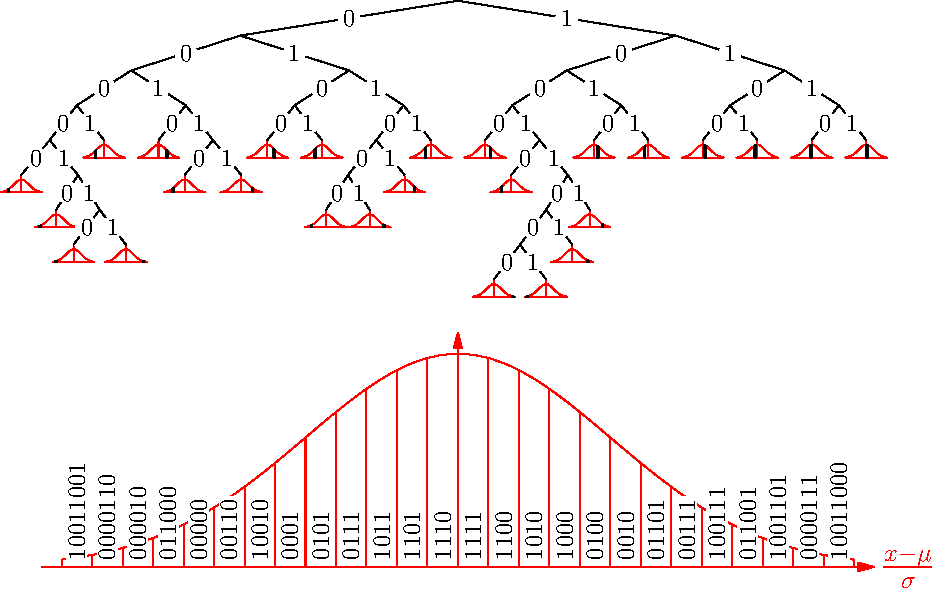
\includegraphics[height=10cm]{huffman}
\end{center}
\keywords{Entropy, Coding, Maximum Entropy}
%%%%%%%%%%%%%%%%%%%%%%% Next Slide %%%%%%%%%%%%%%%%%%%%%%%
\renewcommand{\Outline}{%
\begin{slide}
\section[1]{Outline}

\begin{minipage}{10cm}\raggedright
  \begin{enumerate}\squeeze
    \outlineitem{Measuring Uncertainty}{uncertainty}
    \outlineitem{Code Length}{code}
    \outlineitem{Maximum Entropy}{maxentropy}
  \end{enumerate}
\end{minipage}\hfill
\begin{minipage}{12cm}
  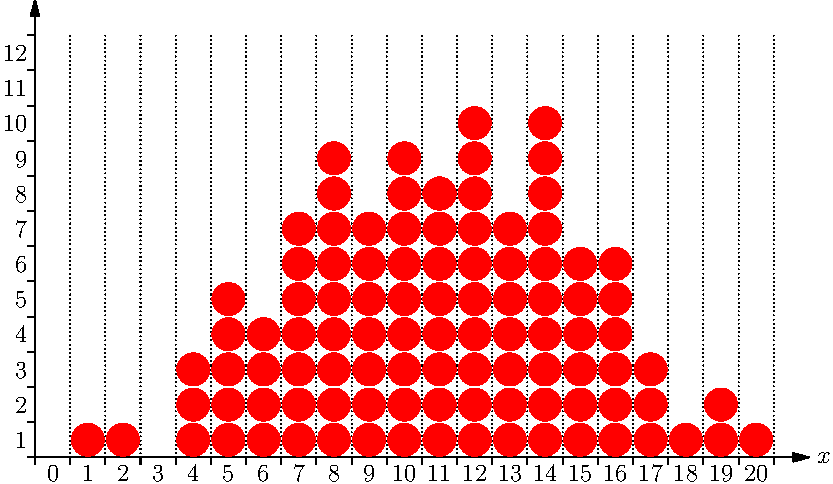
\includegraphics[width=12cm]{maxent}
\end{minipage}
\end{slide}
\addtocounter{outlineitem}{1}
}

\newcommand{\bits}{\,\mathrm{bits}}
\setcounter{outlineitem}{1}
\Outline % Motivation
\toptarget{firstoutline}
%%%%%%%%%%%%%%%%%%%%%%% Next Slide %%%%%%%%%%%%%%%%%%%%%%%

\begin{slide}
\section{Measuring Uncertainty}
  
\begin{PauseHighLight}
  \begin{itemize}
  \item What is more uncertain: tossing a coin three times or throwing
    a dice?\pause
  \item The answer depends on whether you care about the order of the
    coin tosses\pause
  \item But, how do we answer such a question?\pause
  \item Let $X$ be a random variable denoting the possible outcomes\pause
  \item Interestingly, Shannon entropy gives a precise answer
    \begin{align*}
      H_X = -\sum_{x\in\mathcal{X}} \Prob{X=x}\, \logtwo{\Prob{X=x}}\pause
    \end{align*}
  \end{itemize}
\end{PauseHighLight}

\end{slide}

%%%%%%%%%%%%%%%%%%%%%%% Next Slide %%%%%%%%%%%%%%%%%%%%%%%

\begin{slide}
\section{Let's Calculate}

\begin{PauseHighLight}
  \begin{itemize}
  \item For an honest dice $D \in\{1,2,3,4,5,6\}$ and $\Prob{D=i} = 1/6$
    so
    \begin{align*}
      H_D = - \sum_{i=1}^6 \frac{1}{6} \logtwo{ \frac{1}{6}} = - \logtwo{
      \frac{1}{6}} = \log_2(6) \approx 2.585 \bits\pause
    \end{align*}
  \item For an honest coin where we care about the order so $C \in
    \{000,001,\ldots, 111\}$ the $\Prob{C=i} = \frac{1}{8}$ and
    \begin{align*}
      H_C = - \sum_{i=0}^7 \frac{1}{8} \logtwo{ \frac{1}{8}} = - \logtwo{
      \frac{1}{8}} = \log_2(8) = 3 \bits\pause
    \end{align*}
  \item This clearly makes sense: there are more possible outcomes; all
    equally likely\pause
  \end{itemize}
\end{PauseHighLight}


\end{slide}

%%%%%%%%%%%%%%%%%%%%%%% Next Slide %%%%%%%%%%%%%%%%%%%%%%%

\begin{slide}
\section{Unordered Coin Toss}

\begin{PauseHighLight}
  \begin{itemize}
  \item What if we don't care about the order of the outcome?  Then
    $\Prob{HHH}=\Prob{TTT}=1/8$, while two heads (or two tails) in any
    order have $\Prob{HHT}=\Prob{HTT}=3/8$ so
    \begin{align*}
      H_U = -\frac{1}{4} \logtwo{\frac{1}{8}} - \frac{3}{4}
      \logtwo{\frac{3}{8}}\approx 1.811 \bits\pause
    \end{align*}
  \item This seems reasonable, although it is not obvious how you
    would determine this without using entropy\pause
  \item But why Shannon entropy?\pauseb
  \end{itemize}
\end{PauseHighLight}

\end{slide}

%%%%%%%%%%%%%%%%%%%%%%% Next Slide %%%%%%%%%%%%%%%%%%%%%%%

\begin{slide}
\section[-2]{Additive Entropy}

\begin{PauseHighLight}
  \begin{itemize}
  \item If $H_X$ and $H_Y$ are the uncertainties of two independent random
    variables $X$ and $Y$, what is the uncertainty of the combined
    event $(X,Y)$?
    \begin{align*}
      H_{(X,Y)}
      &= -\sum_{X,Y} \Prob{X,Y} \, \logtwo{\Prob{X, Y}}\pause\\
      &= -\sum_{X,Y} \Prob{X}\Prob{Y} \, \logtwo{\Prob{X} \Prob{Y}}\pause\\
      &= -\sum_{X,Y} \Prob{X}\Prob{Y} \,\left(  \strut\logtwo{\Prob{X}}+
        \logtwo{\Prob{Y}} \right)\pause\\
      &= -\sum_X \Prob{X}\,\logtwo{\Prob{X}} - \sum_Y
        \Prob{Y}\,\logtwo{\Prob{Y}}\pause
        = H_X + H_Y\pause
    \end{align*}
  \item With a few other natural requirements, Shannon's entropy is
    the only function with this property\pause
  \end{itemize}
\end{PauseHighLight}

\end{slide}


%%%%%%%%%%%%%%%%%%%%%%% Next Slide %%%%%%%%%%%%%%%%%%%%%%%
\Outline % Code Length
%%%%%%%%%%%%%%%%%%%%%%% Next Slide %%%%%%%%%%%%%%%%%%%%%%%

\begin{slide}
\section[-2]{Why Measure Entropy in Bits}
  
\begin{PauseHighLight}
  \begin{itemize}
  \item Suppose we had to communicate a message with $2^n$ equally
    likely outputs (e.g. the result of $n$-coin tosses)\pause
  \item We can do this with a binary string with $n$ bits
    (011..0)\pause
  \item If there were 5 possible outcomes I could do this with 3 bits,
    but waste 3/8 of the message\pause
  \item However if we have a batch of 3 independent messages each with 5
    outcomes then there are 125 possible outcomes\pause.  We could communicate
    this with 7 bits ($2^7=128$), wasting only 3/128 of the
    message\pauseb
  \item By batching together enough messages  with $N$ outcomes then
    we asymptotically  need just $\log_2(N)$ bits\pause
  \end{itemize}
\end{PauseHighLight}

\end{slide}

%%%%%%%%%%%%%%%%%%%%%%% Next Slide %%%%%%%%%%%%%%%%%%%%%%%

\begin{slide}
\section[-2]{Different Probabilities}

\pb
  \begin{itemize}
  \item We ``showed'' that if we had $N$ events, $X_i$, each with
    probability, $\Prob{X_i} = 1/N$, we can code the outcomes with a
    message of length $-\logtwo{\Prob{X_i}}\pause=\logtwo{N}$\pauseb
  \item With a shorter message we would not be able to distinguish all
    possible outcomes from the message\pauseh
  \item What happens if some of the outcomes occur with a different probability\pauseh \pauselevel{=1, =2, =3}
    \begin{center}
      \multipdf[width=0.9\linewidth]{diceEntropy}\pause
    \end{center}
  \end{itemize}

\end{slide}

%%%%%%%%%%%%%%%%%%%%%%% Next Slide %%%%%%%%%%%%%%%%%%%%%%%

\begin{slide}
\section[-1]{Shannon's Entropy}

\begin{PauseHighLight}
  \begin{itemize}
  \item If the probabilities are not equal to $2^{-n}$ we can
    still find a code with a length very close to $-\logtwo{\Prob{X}}$
    per message by transmitting a large number of messages\pause
  \item The length of the message measures the amount of
    \emph{surprise} on receiving the message\pause
  \item Shannon's entropy is the minimum expected length of the message
    to communicate a random variable $X$
    \begin{align*}
      H_X = \av[X]{-\logtwo{\Prob{X}}}
      = - \sum_{x\in\mathcal{X}} \Prob{X=x}\, \logtwo{\Prob{X=x}}\pause
    \end{align*}
  \item The expected length is a measure of the uncertainty\pause{} (how much
    information on average we need to convey the outcome)\pauseb
  \end{itemize}
\end{PauseHighLight}
  

\end{slide}

%%%%%%%%%%%%%%%%%%%%%%% Next Slide %%%%%%%%%%%%%%%%%%%%%%%

\begin{slide}
\section[-1]{Real Codes}

\begin{PauseHighLight}
  \begin{itemize}
  \item Those of you with some computer science background will
    realise that with code words of different lengths we must know
    where each code word ends\pause
  \item A \emph{prefix code} (no code word is the start of another)
    can always be decoded\pause
  \item An optimal prefix code is Huffman encoding where we
    associate the leaf of a tree with each code word\pause{} (its
    expected length is between $H_X$ and $H_X+1$ bits)\pauseb
  \item Using the tree we can decode any message constructed using the
    tree\pause
  \item There is a greedy algorithm for constructing the optimal
    tree\pause
  \end{itemize}
\end{PauseHighLight}

\end{slide}

%%%%%%%%%%%%%%%%%%%%%%% Next Slide %%%%%%%%%%%%%%%%%%%%%%%

\begin{slide}
\section[-2]{Coding Normals}

\begin{center}
  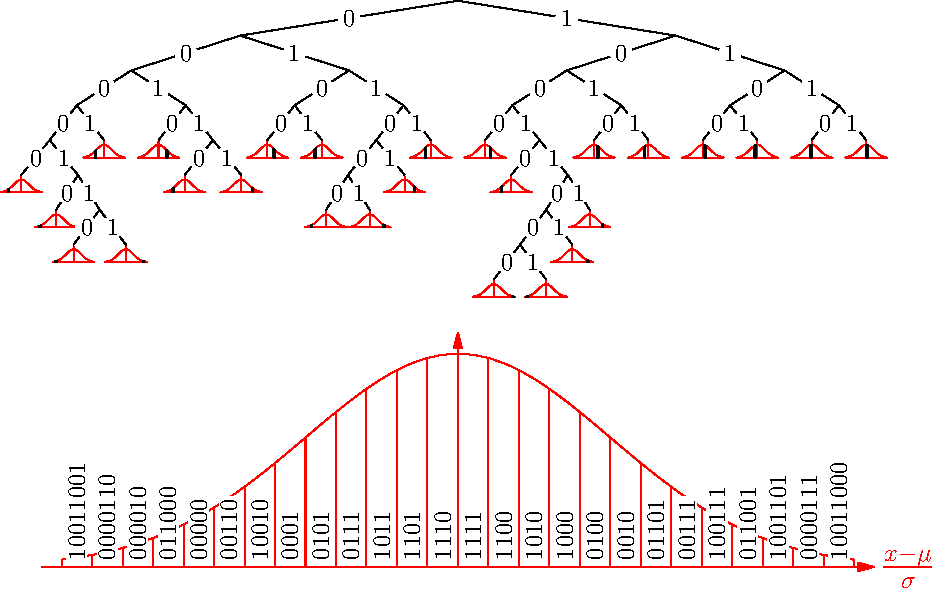
\includegraphics[width=\linewidth]{huffman}
\end{center}
\end{slide}

%%%%%%%%%%%%%%%%%%%%%%% Next Slide %%%%%%%%%%%%%%%%%%%%%%%

\begin{slide}
\section{Coding Normals to Accuracy $\Delta x$}

\pb \pause \pauselevel{=1}
\begin{center}
  \multipdf[width=0.9\linewidth]{huffman2}\pause
\end{center}
\end{slide}


%%%%%%%%%%%%%%%%%%%%%%% Next Slide %%%%%%%%%%%%%%%%%%%%%%%

\begin{slide}
\section{bits and nats}

\begin{PauseHighLight}
  \begin{itemize}
  \item We have measured entropy in \emph{bits} using
    \begin{align*}
      H_X = - \sum_{x\in\mathcal{X}} \Prob{X=x} \, \logtwo{\strut \Prob{X=x}}\pause
    \end{align*}
  \item Sometimes it is easier to use natural logarithms
    \begin{align*}
      H_X = - \sum_{x\in\mathcal{X}} \Prob{X=x} \, \ln\!\bra{\strut \Prob{X=x}}\pause
    \end{align*}
  \item In this case the entropy is measured in \emph{nats} with 1 nat
    equal to $\log_2(\mathrm{e})$ bits\pause
  \item This is often easier when we want to do calculus on entropy\pause
  \end{itemize}
\end{PauseHighLight}

\end{slide}


%%%%%%%%%%%%%%%%%%%%%%% Next Slide %%%%%%%%%%%%%%%%%%%%%%%
\Outline % Maximum Entropy
%%%%%%%%%%%%%%%%%%%%%%% Next Slide %%%%%%%%%%%%%%%%%%%%%%%

\begin{slide}
\section[-2]{Number of States}

\begin{PauseHighLight}
  \begin{itemize}
  \item Suppose I have $N$ balls and put them in $K$ boxes so that $n_i$
    balls finish up in box $i$
    \begin{center}
      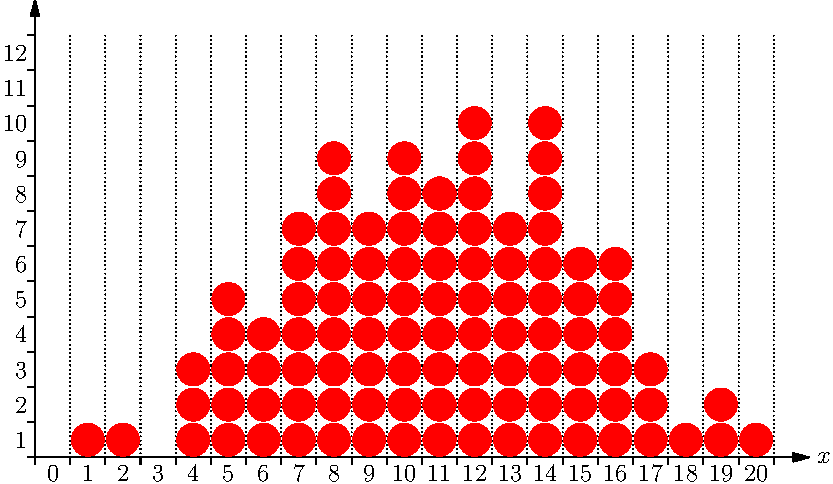
\includegraphics[width=0.6\linewidth]{maxent}
    \end{center}
  \item Counting the number of ways to do this
    \begin{align*}
      W(\bm{n}) &= \frac{N!}{n_1!\,n_2!\cdots n_K!}\pause
    \end{align*}
  \end{itemize}
\end{PauseHighLight}

\end{slide}

%%%%%%%%%%%%%%%%%%%%%%% Next Slide %%%%%%%%%%%%%%%%%%%%%%%

\begin{slide}
\section[0]{Stirling's Approximation}

\begin{rightImage}[0.2]{stirling}
  \begin{PauseHighLight}
  \small
  \begin{itemize}
  \item We can approximate the factorial $n!$ using \emph{Stirling's
      approximation}
    \begin{align*}
      n! &\approx \sqrt{2\,\pi\,n}\, n^n\,\e{-n} \\
      \log(n!) &\approx n \log(n) - n + \frac{1}{2}\log(2\,\pi\,n)\pause
    \end{align*}
  \item Using this in our formula for $W(\bm{n})$ we have
    \begin{align*}
      W(\bm{n})&= \frac{N!}{n_1!\,n_2!\cdots n_K!} \pause
                     = \e{\log(N!) - \sum\limits_i \log(n_i!)} \pauseb \\
                     &\approx C\, \e{N\,\log(N) - \sum\limits_i n_i
                       \log(n_i)} \pauseb
                       \approx C \, \e{- N \sum\limits_i \frac{n_i}{N}
      \logg{\frac{n_i}{N}} }\pauseb
    \end{align*}
    \pauselevel{=4} Order $n$ terms cancel as $N=\sum\limits_i n_i$ \pauseb
  \end{itemize}
  \end{PauseHighLight}
\end{rightImage}
\end{slide}

%%%%%%%%%%%%%%%%%%%%%%% Next Slide %%%%%%%%%%%%%%%%%%%%%%%

\begin{slide}
\section[-2]{Number of States and Entropy}
  
\begin{PauseHighLight}
  \begin{itemize}
  \item Let $p(x_i) = n_i/N$ be the proportion of balls in bin $i$ then
    \begin{align*}
      W(\bm{n}) \approx C \e{N\,H_X}
    \end{align*}
    where
    \begin{align*}
      H_X = -\sum_{i} p(x_i)\, \logg{p(x_i)}\pause
    \end{align*}
  \item That is, the ``entropy'' can be seen as a measure of the
    logarithm of the number of configurations\pause
  \item As the number of balls, $N\rightarrow\infty$, the
    overwhelmingly likely configuration is the one that maximises the
    entropy subject to what we know (e.g.\ an observed mean)\pause
  \end{itemize}
\end{PauseHighLight}

\end{slide}

%%%%%%%%%%%%%%%%%%%%%%% Next Slide %%%%%%%%%%%%%%%%%%%%%%%

\begin{slide}
\section[-2]{Entropy Is Concave}

\begin{PauseHighLight}
  \begin{itemize}\squeeze
  \item Each term $h(p) = -p\ln(p)$ has $h''(p) = -1/p < 0$, so the
    entropy $H = \sum_i h(p_i)$ is a concave function of the
    probabilities\pause{} ($-H$ is convex)\pauseb
  \item Jensen's inequality (convexity lecture) with the concave
    $\log$ gives, for $K$ outcomes,
    \begin{align*}
      H_X = \av{\logtwo{\frac{1}{\Prob{X}}}} \leq
      \logtwo{\av{\frac{1}{\Prob{X}}}} = \log_2(K)\pause
    \end{align*}
    with equality for the uniform distribution\pause
  \item With linear constraints (fixed averages) the maximum entropy
    solution is unique\pause
  \item $-H$ is a convex regulariser favouring spread-out
    distributions (used in optimal transport)\pause
  \end{itemize}
\end{PauseHighLight}

\end{slide}

%%%%%%%%%%%%%%%%%%%%%%% Next Slide %%%%%%%%%%%%%%%%%%%%%%%

\begin{slide}
\section{Maximum Entropy Method}

\begin{PauseHighLight}
  \begin{itemize}
  \item When we are trying to infer a distribution given some
    observations then we can maximise the entropy subject to
    constraints\pause---the entropy acts as a prior\pauseb
  \item This is known as the \emph{maximum entropy method}\pause
  \item We can rationalise this as this is by far the most likely set
    of configurations consistent with the observations\pause
  \item Alternatively we can see this as maximising our uncertainty
    given what we know\pause---being as unbiased as possible\pauseb
  \item It assumes that, before we impose the constraints, every
    configuration is equally likely\pause
  \end{itemize}
\end{PauseHighLight}

\end{slide}

%%%%%%%%%%%%%%%%%%%%%%% Next Slide %%%%%%%%%%%%%%%%%%%%%%%

\begin{slide}
\section[-2]{Knowing the Mean and Variance}

\begin{PauseHighLight}\small
  \begin{itemize}
  \item Consider a continuous random variable, $X$, with a known mean and
    second moment
    \vspace*{-2cm}
    
    \begin{align*}
      \av{X} &= \mu, & \av{X^2} &= \mu_2 = \mu^2 + \sigma^2\pause
    \end{align*}
    \vspace*{-2cm}
    
  \item To maximise the entropy subject to constraints consider
    \vspace*{-1.5cm}
    
    \begin{align*}
      \mathcal{L}(f) &= -\int f_X(x) \, \logg{f_X(x)} \, \dd x +
                       \lambda_0  \left( \int f_X(x) \, \dd x-1 \right)
      \\
                     &\quad + \lambda_1  \left( \int f_X(x)\, x \, \dd x-\mu\right) +
                       \lambda_2  \left( \int f_X(x)\, x^2 \, \dd x-\mu_2\right)\pause
    \end{align*}
    \vspace*{-2cm}
    
  \item Thus
    \vspace*{-2cm}

    \begin{align*}
      \frac{\delta \mathcal{L}(f)}{\delta f_X(x)} =  - \logg{f_X(x)} -1
      + \lambda_0 + \lambda_1\, x + \lambda_2\, x^2 = 0\pause
    \end{align*}
  \item Or
    \begin{align*}
      f_X(x) &= \e{-1 + \lambda_0 + \lambda_1\, x + \lambda_2\, x^2}\pause
    \end{align*}
  \end{itemize}
\end{PauseHighLight}

\end{slide}

%%%%%%%%%%%%%%%%%%%%%%% Next Slide %%%%%%%%%%%%%%%%%%%%%%%

\begin{slide}
\section[-2]{Normal Distribution}
  
\begin{PauseHighLight}\small
  \begin{itemize}
  \item We have three constraints
    \begin{align*}
      \int \e{-1 + \lambda_0 + \lambda_1\, x + \lambda_2\, x^2} \,\dd x &= 1
      \\
      \int \e{-1 + \lambda_0 + \lambda_1\, x + \lambda_2\, x^2} \,x\, \dd x
                                                                        &= \mu \\
      \int \e{-1 + \lambda_0 + \lambda_1\, x + \lambda_2\, x^2} \,x^2\, \dd
      x &= \mu_2 =  \mu^2 + \sigma^2\pause
    \end{align*}
  \item Solving for $\lambda_0$, $\lambda_1$ and $\lambda_2$ then
     \begin{align*}
       f_X(x) = \frac{1}{\sqrt{2\,\pi}\, \sigma} \e{-(x-\mu)^2/(2\sigma^2)}\pause
     \end{align*}
   \item That is, the normal distribution is the maximum entropy
     distribution given we know the mean and variance\pause
  \end{itemize}
\end{PauseHighLight}

\end{slide}

%%%%%%%%%%%%%%%%%%%%%%% Next Slide %%%%%%%%%%%%%%%%%%%%%%%

\begin{slide}
\section[-2]{Softmax Is Maximum Entropy}

\begin{PauseHighLight}\small
  \begin{itemize}
  \item A model gives scores $s_i$ to $K$ classes; find the
    probabilities $p_i$ with maximum entropy and a given average score
    $\sum_i p_i\,s_i = \bar{s}$\pause
  \item As for the normal distribution, use Lagrange multipliers
    \begin{align*}
      \mathcal{L} = -\sum_i p_i \ln(p_i) + \lambda_0\Bigl(\sum_i p_i -1\Bigr)
      + \beta\Bigl(\sum_i p_i\, s_i - \bar{s}\Bigr)\pause
    \end{align*}
  \item Setting $\partial\mathcal{L}/\partial p_i = -\ln(p_i) - 1 +
    \lambda_0 + \beta\,s_i = 0$ gives the \emph{softmax}
    \begin{align*}
      p_i = \frac{\e{s_i/T}}{\sum_j \e{s_j/T}}, \qquad T = 1/\beta\pause
    \end{align*}
  \item The temperature $T$ is (the inverse of) a Lagrange multiplier,
    as in statistical physics\pause{}; it is the ``temperature'' used
    when sampling from language models\pauseb
  \item With scores $s_i = \bm{w}_i^\tr\bm{x}$ this is multinomial
    logistic regression, also called the maximum entropy
    classifier\pause
  \end{itemize}
\end{PauseHighLight}

\end{slide}


%%%%%%%%%%%%%%%%%%%%%%% Next Slide %%%%%%%%%%%%%%%%%%%%%%%

\begin{slide}
\section{Using Maximum Entropy}

\begin{PauseHighLight}
  \begin{itemize}
  \item Maximum entropy is often used to infer distributions\pause
  \item It can be very effective, but it might not work well if there are
    other constraints that we have not included\pause
  \item The place that they work superbly well is in statistical
    physics\pause
  \item The whole of statistical physics is about inferring
    distributions making observations of volume, pressure, etc.\pause
  \item Temperature appears rather strangely as a Lagrange multiplier\pause
  \end{itemize}
\end{PauseHighLight}

\end{slide}

%%%%%%%%%%%%%%%%%%%%%%% Next Slide %%%%%%%%%%%%%%%%%%%%%%%

\begin{slide}
\section[-1]{Historic Entropy}

\begin{PauseHighLight}
  \begin{itemize}
  \item Historically entropy was first introduced in statistical
    physics by Rudolf Clausius in 1865 (although Macquorn Rankine
    discussed it in 1850)\pause
  \item Its interpretation as the number of states was introduced by
    Ludwig Boltzmann\pause
  \item The person who got it all right was Josiah Willard Gibbs (and
    James Clerk Maxwell)\pause
  \item Claude Shannon invented information theory based on entropy
    around 1948 (more on that in the next lecture)\pause
  \item Ed Jaynes was the first to understand that statistical physics
    can be seen as an inference problem\pause
  \end{itemize}
\end{PauseHighLight}

\end{slide}

%%%%%%%%%%%%%%%%%%%%%%% Next Slide %%%%%%%%%%%%%%%%%%%%%%%

\begin{slide}
\section{Conclusion}

\begin{PauseHighLight}
  \begin{itemize}
  \item Entropy provides a measure of the disorder or uncertainty in a
    system\pause
  \item It forms the basis of information theory which we will look at
    in the next lecture\pause
  \item $-\log(\Prob{X=x})$ can be seen as the minimum length of a
    message to communicate $x$\pause
  \item This will be used as the basis of the minimum description
    length formalism also discussed in the next lecture\pause
  \item Entropy can be used as a prior, which we often maximise
    subject to constraints to obtain an unbiased estimate\pause
  \end{itemize}
\end{PauseHighLight}

\end{slide}




%%% Local Variables:
%%% TeX-master: "lectures"
%%% End:

\end{document}
